\begin{frame}[allowframebreaks,allowdisplaybreaks]
    \subsection[The Alpha and Beta Constant]{The \texorpdfstring{\(\alpha\)}{alpha} \& \texorpdfstring{\(\beta\)}{beta} Constants}
    \frametitle{AB-Tree The \(\alpha\) \& \(\beta\) constants}
    \begin{columns}
        \begin{column}{\textlecolumn}
            \begin{block}{}
                \begin{itemize}
                    \item As stated the \(\alpha\) in a B-Tree, a predefined constant, defines the \emph{Branching factor} of the tree.
                    \item Likewise the \(\alpha\) and \(\beta\) of a AB-Tree, both predefined constants, will define the \emph{Branching factor} of the tree.
                    \item We define \(\alpha\) and \(\beta\) as natural numbers such that
                        \[
                            \alpha \geq 2 
                            \hspace{1cm}
                            \beta \geq 2 \alpha - 1
                        \]
                    Which, as stated before, are the bounds of the \(\alpha\) constant in some definitions of the B-Tree.
                    \item Since the AB-Tree and B-Tree shares the same minimun number of keys and subtrees on a page, 
                        we can use the same lower bound for the height of a AB-Tree.
                    \item But they don't share the maximun number of keys and subtrees on a page, then the upper bound of the height of the AB-Tree will be different.
                \end{itemize}
            \end{block}
        \end{column}
        \begin{column}{\textricolumn}
        \end{column}
    \end{columns}
    \framebreak{}
    \begin{figure}
        \centering
        \includegraphics[
            width=0.95\linewidth,
            keepaspectratio,
            page=11
        ]{resources/made/B-Trees_general.pdf}
        \caption[]{AB-Tree, \(\tau \left(2, 4, 2\right)\)}
    \end{figure}
\end{frame}
